%Template by Morten Espensen
%Deffinere kommandoer til om vores information

\documentclass[]{report}
%\usepackage{color}
%\usepackage{alltt}
\usepackage{amsmath}
\usepackage{amssymb}
\usepackage{float}
\usepackage[parfill]{parskip}
\usepackage{lscape}
\usepackage{enumerate}
\usepackage{amsmath}
\usepackage[danish,english]{babel}

\usepackage[paper=A4,pagesize]{typearea}
\usepackage[toc,page]{appendix}

\usepackage[utf8]{inputenc}
\usepackage{fancyhdr}
%\usepackage{boxproof}
%\usepackage{daymonthyear}
\usepackage{stmaryrd}

\usepackage{color}
\usepackage{fancyvrb}
\usepackage[usenames,dvipsnames]{xcolor}
\fvset{frame=single,framesep=1mm,fontfamily=courier,fontsize=\scriptsize,numbers=left,framerule=.3mm,numbersep=1mm,commandchars=\\\{\}}

\usepackage{wallpaper} % For the frontpage background

\usepackage{listings} % KODE SHIT
\lstset{ %
language=PHP,          		    % the language of the code
basicstyle=\footnotesize,       % the size of the fonts that are used for the code
numbers=left,                   % where to put the line-numbers
numberstyle=\footnotesize,      % the size of the fonts that are used for the line-numbers
stepnumber=1,                   % the step between two line-numbers. If it's 1, each line
                                % will be numbered
numbersep=5pt,                  % how far the line-numbers are from the code
backgroundcolor=\color{white},  % choose the background color. You must add \usepackage{color}
showspaces=false,               % show spaces adding particular underscores
showstringspaces=false,         % underline spaces within strings
showtabs=false,                 % show tabs within strings adding particular underscores
frame=single,                   % adds a frame around the code
tabsize=2,                      % sets default tabsize to 2 spaces
captionpos=b,                   % sets the caption-position to bottom
breaklines=true,                % sets automatic line breaking
breakatwhitespace=false,        % sets if automatic breaks should only happen at whitespace
title=\lstname,                 % show the filename of files included with \lstinputlisting;
                                % also try caption instead of title
escapeinside={\%*}{*)},         % if you want to add a comment within your code
morekeywords={*,...,xchar,xstring,xmany1,chainl1,chainl1',ReadP}            % if you want to add more keywords to the set
}

\newcommand{\theassingment}{Development of E-learning concept\\[1.6ex]for Medical Personnel}
\newcommand{\thesubassignment}{Innovation phase report}
\newcommand{\shorttheassingment}{ITIC}
%\newcommand{\thepaperauthor}{}
\newcommand{\personalid}{dzr440 - 19/06/1991}
\newcommand{\thesubject}{IT Innovation and Change}
\newcommand{\theinstitute}{Department of Computer Science}
\newcommand{\thesupervisor}{Cosmin E. Oancea} %behøves kun hvis findes

\newcommand*{\diffdchar}{\mathrm{d}}    % or {ⅆ}, or {\mathrm{d}}, or whatever standard you’d like to adhere to
\newcommand*{\dd}{\mathop{\diffdchar\!}}

\newenvironment{timesfont}{\fontfamily{mathptmx}\selectfont}{}

\setlength\parskip{2ex}
\newcommand{\n}[0]{\\[2ex]} %NEWLINE [2ex]
\newcommand{\set}[1]{\{#1\}}
\usepackage{hyperref}

\newcommand{\fnurl}[2]{\href{#2}{#1}\footnote{\url{#2}}}  %foodnote url ref \fnurl{String}{Link}

\newcommand{\premise}{\=\mbox{premise}}
\newcommand{\assumption}{\=\mbox{assumption}}
\newcommand{\landi}{\=\intro\land : }
\newcommand{\lande}{\=\elim\land_{1} : }
\newcommand{\landee}{\=\elim\land_{2} : }
\newcommand{\lori}{\=\intro\lor_{1} : }
\newcommand{\lorii}{\=\intro\lor_{2} : }
\newcommand{\lore}{\=\elim\lor : }
\newcommand{\toi}{\=\intro\to : }
\newcommand{\toe}{\=\elim\to : }
\newcommand{\lnoti}{\=\intro\lnot : }
\newcommand{\lnote}{\=\elim\lnot : }
\newcommand{\bote}{\=\elim\bot : }
\newcommand{\lnege}{\=\lnot\elim\lnot : }
\newcommand{\lnegi}{\=\lnot\intro\lnot : }
\newcommand{\leqi}{\= \intro= }
\newcommand{\leqe}{\= \elim= : }
\newcommand{\lforalli}{\= \intro\forall : }
\newcommand{\lforalle}{\= \elim\forall : }
\newcommand{\lexistsi}{\= \intro\exists : }
\newcommand{\lexistse}{\= \elim\exists : }
\newcommand{\MT}{\=MT : }
\newcommand{\PBC}{\=PBC : }
\newcommand{\LEM}{\=LEM : }

\newenvironment{changemargin}[1]{
  \begin{list}{}{
    \setlength{\voffset}{#1}
  }
  \item[]}{\end{list}}


\usepackage{hyperref}
\usepackage{pdfpages} % til at tilføje apendix
\usepackage{graphicx}
\DeclareGraphicsExtensions{.pdf,.png,.jpg}

\def\thesection{\thechapter.\arabic{section}}
%\renewcommand{\thesubsection} {\thesection.\alph{subsection}}

\pagestyle{fancy}
\fancyhead{}
\fancyhead[LO,LE]{\shorttheassingment}
\fancyhead[RO,RE]{\today}
\fancyhead[CO,CE]{\theinstitute}

\setcounter{secnumdepth}{0}
\setcounter{tocdepth}{3}

\begin{document}
\begin{titlepage}
\begin{timesfont}
% Import the ku frontpage graphics
\ThisULCornerWallPaper{1}{nat-farve.pdf}
% Import faculty title
\ThisULCornerWallPaper{1}{nat-en.pdf}
% For forklaring af vspace og stretch, se side 115 i ".. not so short .."
% www.ctan.org/tex-archive/info/lshort/english/lshort.pdf
\vspace*{3cm}
\hspace*{-2.3cm}
% Her vælger en kæmpe skrifttype og fed skrift
\Huge\bfseries
\vspace*{-0.5cm}
\theassingment\n
\hspace*{-2.4cm}
-- \thesubassignment \n
\LARGE
\hspace*{-2.4cm}
\vspace*{-0.5cm}
\thesubject \\[2.2ex]
\hspace*{-2.4cm}
\vspace*{5.0cm}
\theinstitute \n
\hspace*{-2.38cm}
\large
\textbf{Written by:}\\[1ex]
\hspace*{-2.33cm}
Morten Espensen (dzr440)\\
\hspace*{-2.33cm}
David B. Gandrup (vpd177)\\
\hspace*{-2.33cm}
Sokratis S. Drosos (dnb823)\\
\hspace*{-2.33cm}
Bjarki Madsen (lch929)\\
\hspace*{-2.33cm}
Niklas Høj (nwv762)\\
%\vspace*{1cm}
\hspace*{-2.33cm}
% Nulstiller skriftstørrelse og type (f.eks. fed)
\normalsize
% VEJLEDER INFORMATION I PÅ FORSIDEN?
%\thesubject \n

\hspace*{-2.33cm}
%\textbf{\emph{Supervised by:}}

\hspace*{-2.33cm}
%\thesupervisor

\end{timesfont}
\end{titlepage}
\tableofcontents

\newpage

\section{Methodical approach}
In this phase we analysed the results from our questionnaire that we sent out in the previous phase, performed a SWOT analysis to help us with our decision of what approach of innovation we should use and finally created prototypes to express our visions of change.

\subsection{Questionnaire}
We chose to do a questionnaire as a means of looking into the needs of actual doctors in the DMA since a questionnaire can be more open-ended and insightful than other methods available within our resources. One group of DMA doctors we had access to were those who had participated in the Genetics Course provided by the DMA, which we were also given access to in our case study. Of these, 6 participants consented to participating in our questionnaire. However, at the time of this writing only 2 have responded. Thus our analysis is based on less participants than we would have liked. Another pitfall of this particular study is that we are only focusing on doctors that have been enrolled in a DMA course, and thus there might be a segment of doctors whose perspective is not addressed here.

From our questionnaire we learned the following about the DMA doctors who had participated in the Genetics Course:
\begin{itemize}
\item They find courses for their continuous professional education through Lægeforeningen. Other resources used are Facebook groups, homepages for societies and colleagues.
\item They think courses relevant to their interests are easy to find.
\item They found the DMA Genetics Course very informative and educational (both as new knowledge and as an update on the material).
\item They are at best working full time, and at worst working much more than that. Days have to be taken out of their schedules to attend courses (and that is in one case planned for).
\item They prefer physically attending courses to e-learning (although one had had a good experience with a webinar). Other specific forms of learning mentioned were meetings, congress and reading.
\item They have experienced a couple of e-learning courses but didn't like them.
\item One would like for the DMA to develop and offer courses. The other isn't really interested.
\item They have not tried available e-learning solutions offered such as BMJ and in one case didn't know they existed.
\end{itemize}

\subsection{SWOT}
The reason that we chose to do a SWOT analysis in this phase is because of the very limited time we've had for this phase. We've had many innovative ideas over the course of the design process, some simple and some more complex. To help us with the decision on which idea to choose, we used this technique and chose the innovation, based on the analysis, that had the most strengths and opportunities while having fairly few threats and weaknesses. Figure \ref{fig:swot} shows the identified SWOT attributes of our proposed innovation.

\begin{figure*}[h!]
 \begin{center}
  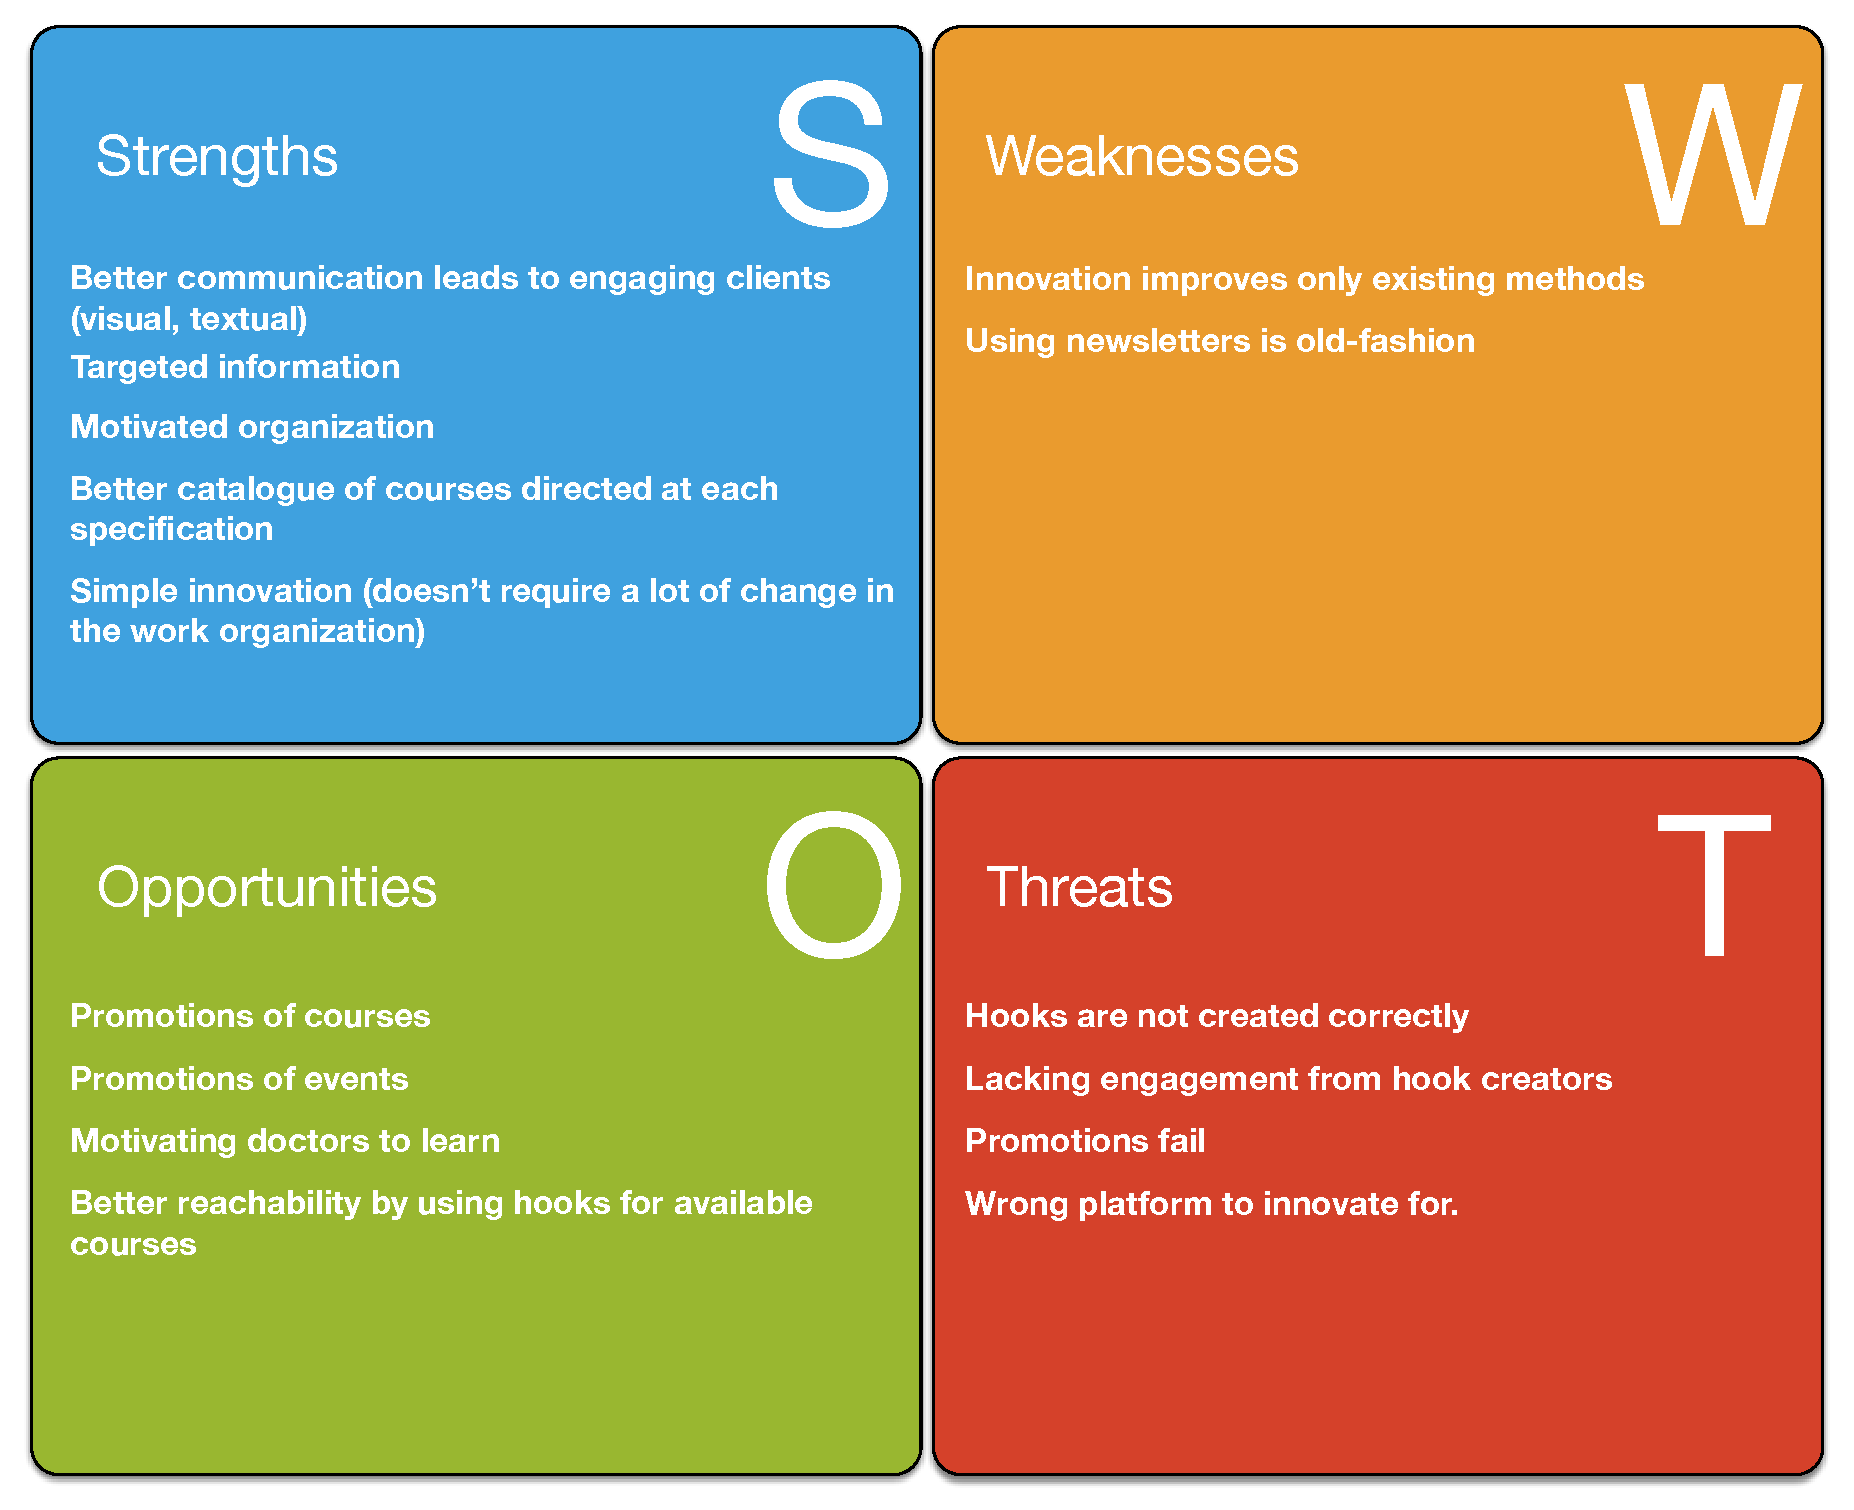
\includegraphics[width=1\textwidth]{figures/swot.pdf}
  \caption{Our SWOT analysis for the innovation stage of the project.\label{fig:swot}}
 \end{center}
\end{figure*}

\section{Innovation phase report}

\subsection{Visions for the overall change}
Our proposed innovation recommends using some of the existing systems available in the organization where we have identified that they play a key role in our innovation. However, we propose an innovative change in how to use and approach these systems.

\textbf{DMA's email newsletter}\\
The email newsletter is an existing system that DMA uses to send their members practical information. From previous phases, we have identified this system to be the key in our innovative solution to engage doctors with e-learning material. The reason for its role in our visions is that it's accessible (i.e it doesn't require a complicated login) and it's perceived as one of the main channel for updates and news.

\textbf{Course Hooks}\\
Our vision of change proposed that to use the newsletter to send out hooks for courses that DMA recommends for different specialities. A hook is a very short video, test or other related media that the doctor can use which allows him/her to get the "sneak peak" of available courses. The hooks are advertised by including exactly how long it takes to watch/read/participate in this "sneak peak" of the course, allowing the doctor to decide if he/she has any spare time for it. These hooks can be created by doctors, course responsibles or even DMA itself.

\textbf{Course Page and Feed}\\
In addition to using the newsletter by promoting courses using hooks, we will also do prototypes using the same terminology which will show how DMA can advertise their courses by using feeds and detail pages (see the prototype section here below). The feed will be personalized based on the doctor's speciality and it will include links to a "landing" page for a course. On the landing page the hook will be the most visible element on the page, whether it's an video, test or other media format.

\subsubsection{IT platform}
The newsletter will continue to use the existing platform and functionality. DMA is currently having an entirely new website developed which will, in our understanding, completely replace the existing website frontend and backend, along with some, if not all, of internal systems also. As we do not currently know the proposed functionality and status of this project, we have chosen to not be too technical in innovation ideas and instead focused on general functions that should be easily implemented on any platform.

\subsubsection{Work organization}
Our vision primarily aims at the work practices at DMA and specifically their role as a course promoter. The email newsletter is a key part of this process and we suggest to keep it like that with some improvements. The work related to putting courses on the website with the suggested course page is also not expected to change much in the work practices at DMA.
Creating the course hook is the biggest change to work practices. Some courses will already have a suitable course hook to use, but it remains to be seen which kind of hook works the best: Videos, other media, tests or very short, concise textual introductions. In either case it could be the responsibility of DMA or the course creator/source to produce this hook.

\subsubsection{Employee qualifications}
For the newsletter and creating course pages no new employee qualifications are needed except the ones dictated by the new IT-platform. For the course hook however, the creator of this needs to know the course and the tool to create the hook. We are suggesting using existing and well known tools and platforms for this, like YouTube for videos and ItsLearning for tests.

\subsection{Costs, advantages and disadvantages}
\subsubsection{The IT systems}
There will be no extra cost in the IT systems because we will be using the already existing IT platform that is also being upgraded, which is the Lægeforeningen website. The advantages would be that course previews on the website will be more appealing to its visitors.

\subsubsection{Work organization and qualification needs}
The extra cost in the work organization would be that either someone has to be hired to create the suggested "hooks" or someone that is already involved in the promotion of the courses must also create the "hooks". That person could be an employee of DMA, the course creators or someone that is promoting the various courses..

In terms of qualification needs, if an external company or employee is hired, it means that they will probably need to be trained to operate, or modify the existing IT systems. In case an existing employee of DMA, or a course creator is assigned to create the hooks there will not be any extra qualification needs.

\subsubsection{The company's business and IT strategies}
As we have stated in the previous section, there will not necessarily be any extra cost in the company business (either new employee, or existing one). The advantages will be that if the course "hooks" work the members of DMA will become more interested in the offered courses and hence continue using their membership in DMA.

In terms of the existing IT strategy, the disadvantage is that the old one will have to be discarded and so it may take some time for the current employees to adapt to the changes proposed by our innovation idea (e.g. train staff to create course "hooks").

\subsection{Implementation strategy and plan}
\subsubsection{Technical}
There are no new technical requirements presented by our solution. As stated earlier the new IT-platform and website dictates the technical possibilities and thus requirements. Our suggestions could help to set up requirements for this new platform.

\subsubsection{Organizational}
Deciding who will be responsible for creating the course hook is the biggest organizational challenge. DMA and the course/learning responsible people there would initially do this, but course "hooks" created by the course source/creator could be preferred.

\subsection{Revised business model canvas}
See figure \ref{fig:bmc_revised}.

\begin{figure*}[h!]
 \begin{center}
  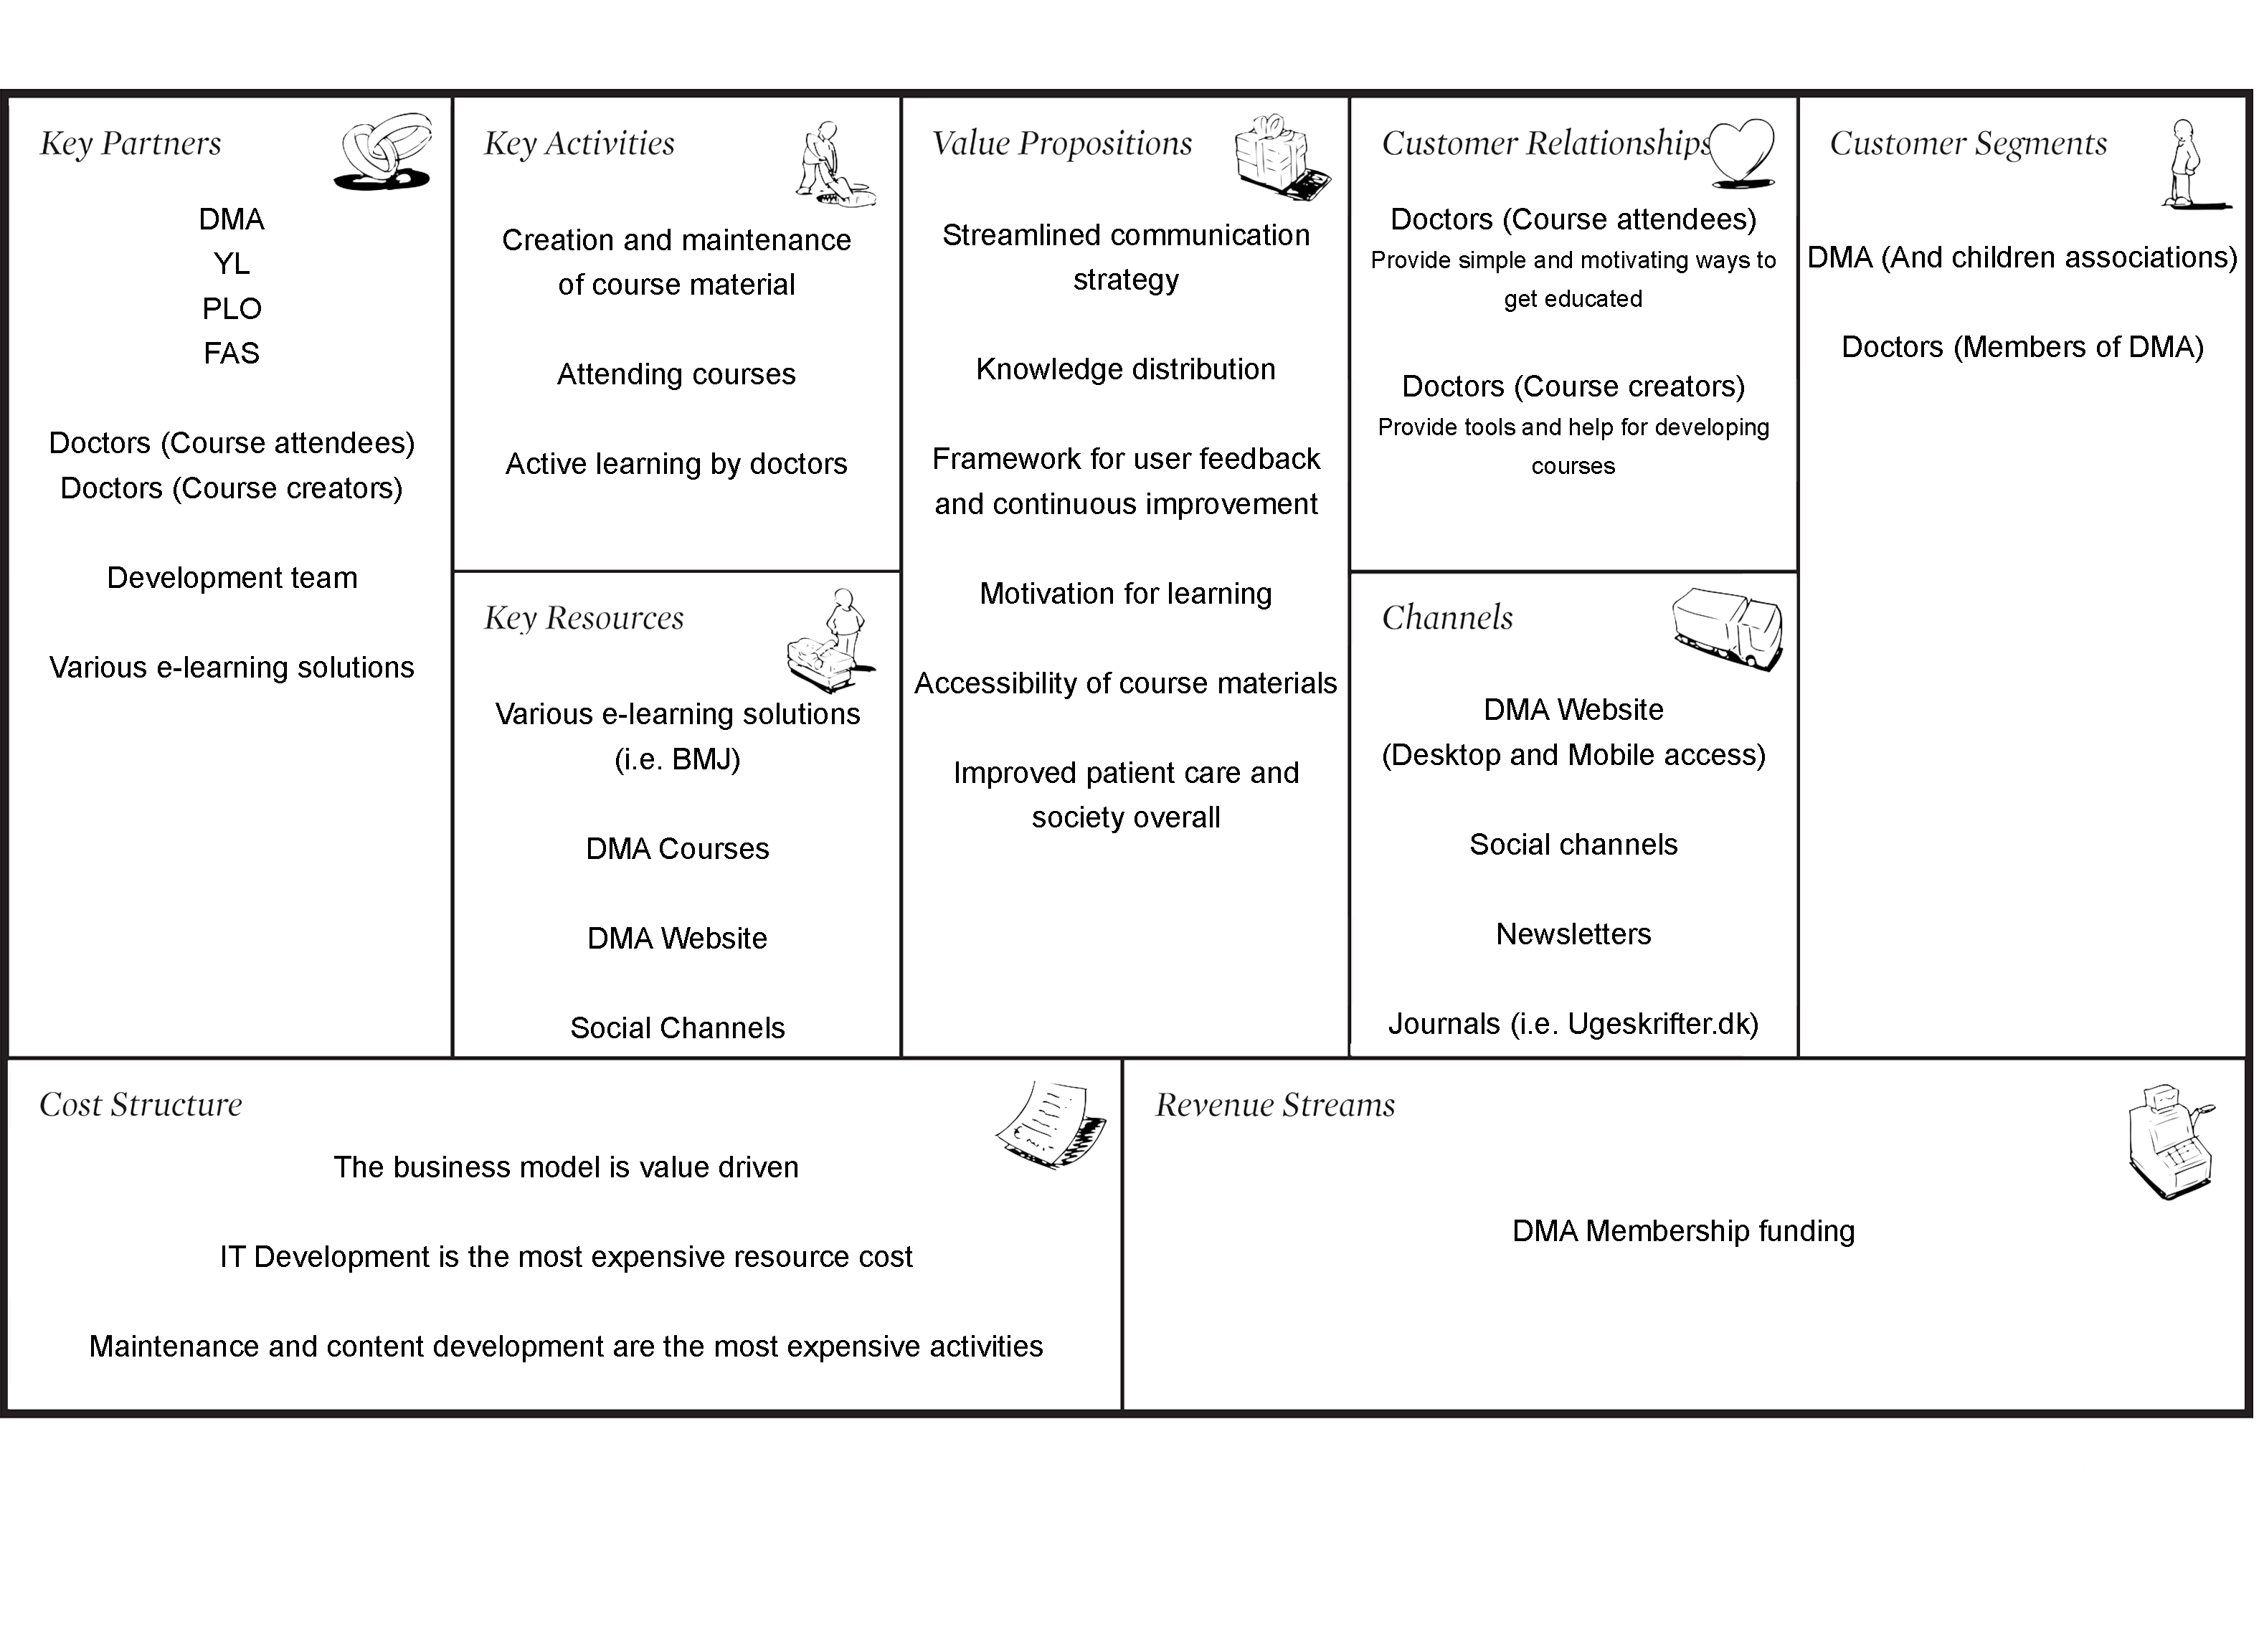
\includegraphics[width=1\textwidth]{figures/Business-Model-Canvas.pdf}
  \caption{Our business model canvas for the project.\label{fig:bmc_revised}}
 \end{center}
\end{figure*}

\subsection{Mock-ups}
We have made a few mock-ups to illustrate how we envision our innovations to be implemented. The main innovation is the "hook" for a course in form of a video, test or other media formats introducing and "selling" the course. Our other innovation is about how this "hook" is presented, made accessible and enticing to watch. In the following we will describe how these are implemented.

\subsubsection{Course page with course hook}
The course page (figure \ref{fig:course_page}) is where the course is presented. This is a page on the new website. The main element of the course page is the embedded course "hook", but the course is also presented in text with relevant information about the course as well as the time it takes to "consume" (watch if it's a video or participate in if it's a test) the hook. Other interesting features of the course page are participant reviews of the course as well as a list of similar courses.

\begin{figure*}[h!]
 \begin{center}
  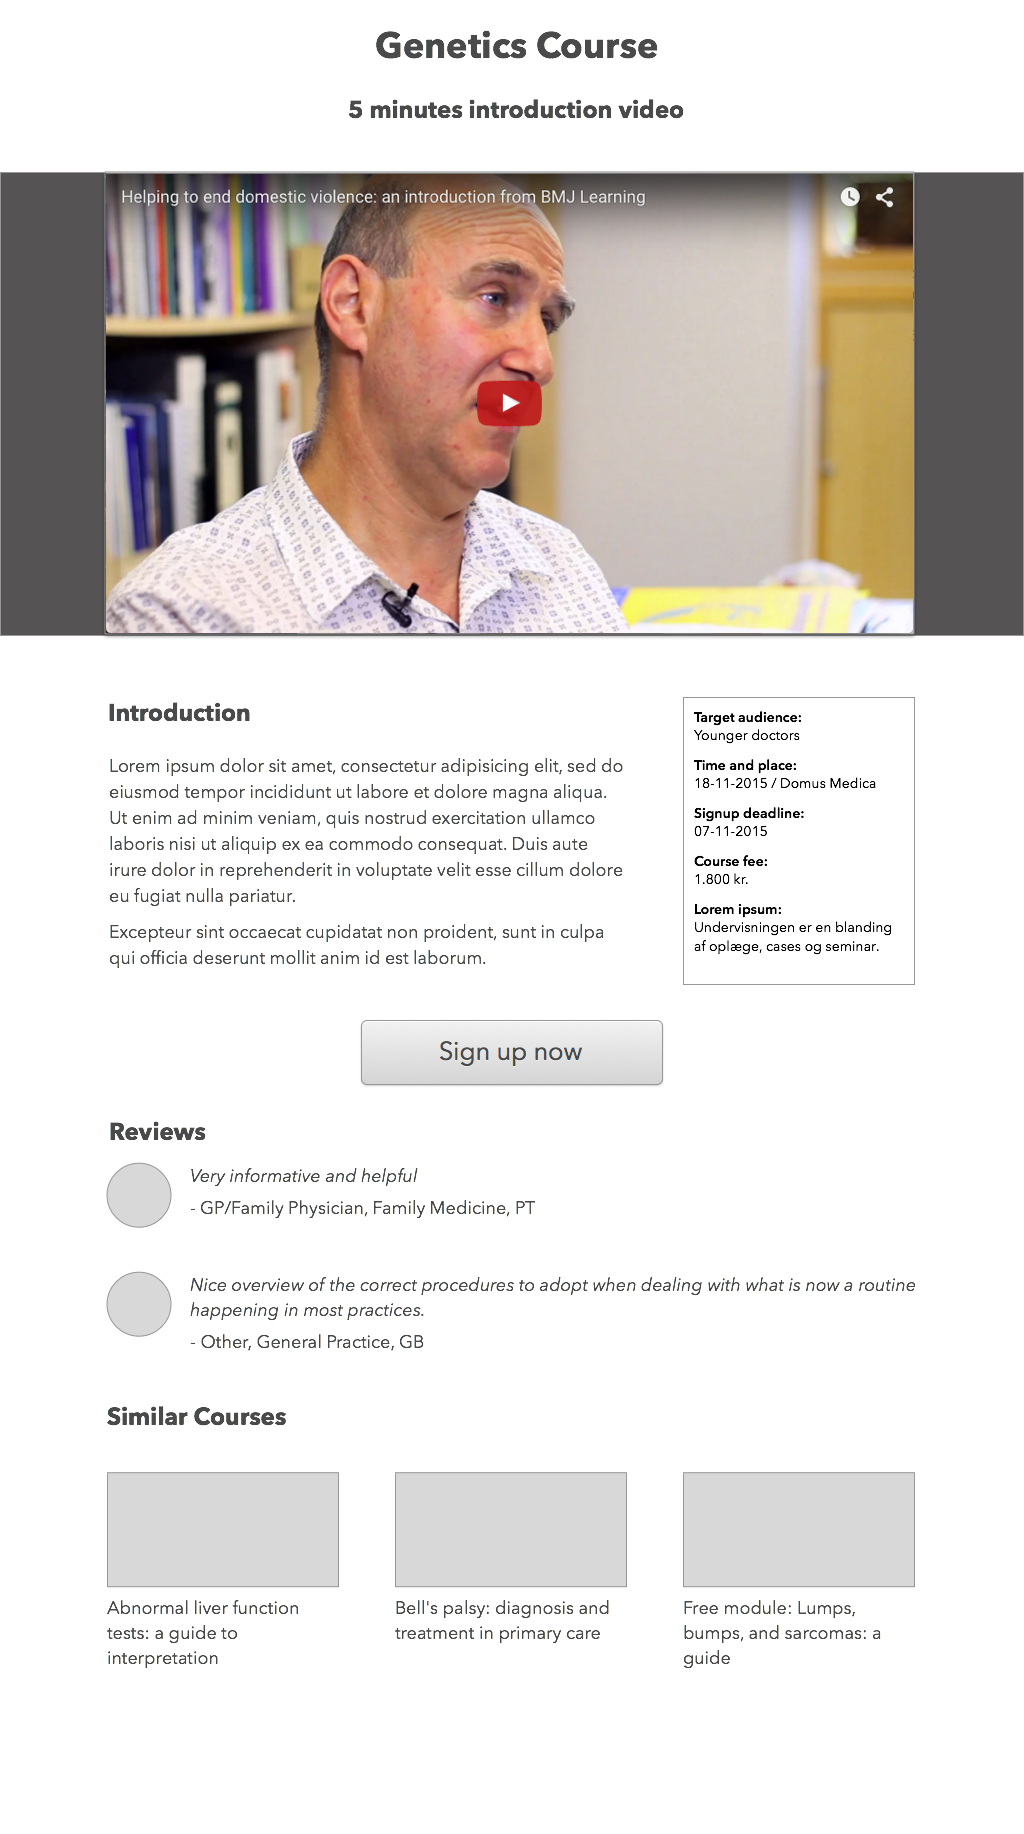
\includegraphics[width=1\textwidth]{figures/course_page_prototype.png}
  \caption{Our mock-up of the course page innovation presenting the course with a course hook and other information.\label{fig:course_page}}
 \end{center}
\end{figure*}

\subsubsection{E-mail newsletter}
DMA currently sends out a newsletter with various news. We would like to add a list of links to the course pages presenting featured courses and their course "hook". Each link should include the name of the course as well as how long the hook takes to consume.

\subsubsection{Course feed}
On the upcoming new website we would like to feature a "course feed". That is, a feed of featured courses where each element in the feed links to the course page containing a course "hook" etc. as described in the course page section above. All featured courses pass through the course feed, and are also stored in a comprehensive history listing of featured courses.







\end{document}
